%!TEX program = xelatex
\documentclass[dvipsnames, svgnames,a4paper,11pt]{article}
% ----------------------------------------------------- 
%	加边框的命令
%	参考:https://tex.stackexchange.com/questions/531559/how-to-add-the-page-border-for-first-two-pages-in-latex
\usepackage{tikz}
\usetikzlibrary{calc}
\usepackage{eso-pic}
\AddToShipoutPictureBG{%
\begin{tikzpicture}[overlay,remember picture]
\draw[line width=0.6pt] % 边框粗细
    ($ (current page.north west) + (0.6cm,-0.6cm) $)
    rectangle
    ($ (current page.south east) + (-0.6cm,0.6cm) $); % 边框位置
\end{tikzpicture}}


\usepackage{xcolor}
\definecolor{c1}{HTML}{070F94} % 目录颜色 原版为2752C9 紫灰色535AAA 蓝紫色0B0DB7 深蓝色070F94 湖绿色219394 松石灰绿086173
\definecolor{c2}{HTML}{E20129} % 引用颜色 原版\definecolor{c2}{RGB}{190,20,83} 橙色F24729

\usepackage{ctex}
\usepackage[top=28mm,bottom=28mm,left=15mm,right=15mm]{geometry}
\usepackage{hyperref} 
\hypersetup{
	colorlinks,
	linktoc = section, % 超链接位置,选项有section, page, all
	linkcolor = c1, % linkcolor 目录颜色
	citecolor = c1  % citecolor 引用颜色
}
\usepackage{amsmath,enumerate,multirow,float}
\usepackage{tabularx}
\usepackage{tabu}
\usepackage{subfig}
\usepackage{fancyhdr}
\usepackage{graphicx}
\usepackage{wrapfig}  
\usepackage{physics}
\usepackage{appendix}
\usepackage{amsfonts}

%
\usepackage{tcolorbox}
\tcbuselibrary{skins,breakable}
\newtcolorbox{tbox}[2][]{
    colframe=black!70!,
    breakable,
    enhanced,
	boxrule =0.5pt,
    title = {#2},
    fonttitle = \large\kaishu\bfseries,
	drop fuzzy shadow,
    #1
}
\newtcolorbox[auto counter,number within=section]{question}[1][]{
  top=2pt,bottom=2pt,arc=1mm,
  boxrule=0.5pt,
%   frame hidden,
  breakable,
  enhanced, %跨页后不会显示下边框
  coltitle=c1!80!gray,
  colframe=c1,
  colback=c1!3!white,
  drop fuzzy shadow,
  title={思考题~\thetcbcounter:\quad},
  fonttitle=\bfseries,
  attach title to upper,
  #1
}

% ---------------------------------------------------------------------
%	利用cleveref改变引用格式,\cref是引用命令
\usepackage{cleveref}
\crefformat{figure}{#2{\textcolor{c2}{Figure #1}}#3} % 图片的引用格式
\crefformat{equation}{#2{(\textcolor{c2}{#1})}#3} % 公式的引用格式
\crefformat{table}{#2{\textcolor{c2}{Table #1}}#3} % 表格的引用格式


% ---------------------------------------------------------------------
%	页眉页脚设置
\fancypagestyle{plain}{\pagestyle{fancy}}
\pagestyle{fancy}
\lhead{\kaishu 中山大学物理与天文学院基础物理实验\uppercase\expandafter{\romannumeral2}} % 左边页眉,学院 + 课程
\rhead{\kaishu 实验报告By黄罗琳} % 右边页眉,实验报告标题
\cfoot{\thepage} % 页脚,中间添加页码


% ---------------------------------------------------------------------
%	对目录、章节标题的设置
\renewcommand{\contentsname}{\centerline{\huge 目录}}
\usepackage{titlesec}
\usepackage{titletoc}
% \titleformat{章节}[形状]{格式}{标题序号}{序号与标题间距}{标题前命令}[标题后命令]
\titleformat{\section}{\centering\LARGE\songti}{}{1em}{}

% ---------------------------------------------------------------------
%   listing代码环境设置
\usepackage{listings}
\lstloadlanguages{python}
\lstdefinestyle{pythonstyle}{
backgroundcolor=\color{gray!5},
language=python,
frameround=tftt,
frame=shadowbox, 
keepspaces=true,
breaklines,
columns=spaceflexible,                   
basicstyle=\ttfamily\small, % 基本文本设置,字体为teletype,大小为scriptsize
keywordstyle=[1]\color{c1}\bfseries, 
keywordstyle=[2]\color{Red!70!black},   
stringstyle=\color{Purple},       
showstringspaces=false,
commentstyle=\ttfamily\scriptsize\color{green!40!black},%注释文本设置,字体为sf,大小为smaller
tabsize=2,
morekeywords={as},
morekeywords=[2]{np, plt, sp},
numbers=left, % 代码行数
numberstyle=\it\tiny\color{gray}, % 代码行数的数字字体设置
stepnumber=1,
rulesepcolor=\color{gray!30!white}
}




% ---------------------------------------------------------------------
%	其他设置
\def\degree{${}^{\circ}$} % 角度
\graphicspath{{./images/}} % 插入图片的相对路径
\allowdisplaybreaks[4]  %允许公式跨页 
\usepackage{lipsum}
\usepackage{enumitem}
\usepackage{tabularray}  %绘制表格时可以更加方便添加框线
\usepackage{xcolor} %添加更多文本颜色
%\usepackage{mathrsfs} % 字体
%\captionsetup[figure]{name=Figure} % 图片形式
%\captionsetup[table]{name=Table} % 表格形式
\begin{document}
	
	% 实验报告封面	
	% 顶栏
	\begin{table}
		\renewcommand\arraystretch{1.7}
		\begin{tabularx}{\textwidth}{
			|>{\centering}X|>{\centering}X|>{\centering}X
			|>{\centering}X|>{\centering}X|>{\centering\arraybackslash}X|}
		\hline
		\multicolumn{2}{|c|}{预习报告}&\multicolumn{2}{c|}{实验记录与分析}&\multicolumn{2}{c|}{总成绩}\\
		\hline
		\LARGE30 & & \LARGE50 & & \LARGE80 & \\
		\hline
		\end{tabularx}
	\end{table}
	
	
	\begin{table}
		\renewcommand\arraystretch{1.7}
		\begin{tabularx}{\textwidth}{|X|X|X|X|}
		\hline
		年级、专业:& 物理学 &组号:& 实验班1\\
		\hline
		姓名:& 黄罗琳 & 学号: & 2344001 \\
		\hline
		日期:& 2024/05/08 & 教师签名:& \\
		\hline
		\end{tabularx}
	\end{table}
	
	\begin{center}
		\LARGE 全息照相实验
	\end{center}
	
	\textbf{【实验报告注意事项】}
	\begin{enumerate}[label=\arabic*., leftmargin=*]
		\item 实验报告由两部分组成:
			\begin{enumerate}[label=\arabic*), leftmargin=*]
				\item 预习报告:课前认真研读\underline{\textbf{实验讲义}},弄清实验原理;实验所需的仪器设备、用具及其使用、完成课前预习思考题;了解实验需要测量的物理量,并根据要求提前准备实验记录表格(可以参考实验报告模板,可以打印)。\textcolor{red}{\textbf{(30分)}}
				\item 实验记录与分析:认真、客观记录实验条件、实验过程中的现象以及数据。实验记录请用珠笔或者钢笔书写并签名(\textcolor{red}{\textbf{用铅笔记录的被认为无效}})。\textcolor{red}{\textbf{保持原始记录,包括写错删除部分,如因误记需要修改记录,必须按规范修改。}}(不得手记的值输入到电脑打印);离开前请实验教师检查记录并签名。\textcolor{red}{\textbf{(50分)}}
			\end{enumerate}
		
		\item \textcolor{red}{\textbf{本实验报告可提前打印出来,当场记录分析完成交给带实验的老师,课后无需再提交。若当场完成不了,则请课后完成,再扫描并通过seelight提交。}}
		
		\textcolor{red}{\textbf{注意:本文档已留出填写空间,若填写空间不够的话请提前规划留白,做到报告的美观}}
		\item 注意事项:
			\begin{enumerate}[label=\arabic*), leftmargin=*]
				\item 实验中\textcolor{red}{\textbf{避免激光器伤到眼睛}}
				\item 避免用手直接接触镜片的光学面
				\item 安装镜片时需在光学平台上尽量靠近台面的高度操作,以免失手跌落摔碎镜片
				\item 实验平台配件所用固定螺钉需拧紧,以免镜架晃动;但不可过紧,以免损坏
				\item 实验前需按仪器清单检查光学元件是否齐全,\textcolor{red}{\textbf{实验结束后按照顺序放回元件盒}}
				
			\end{enumerate}
	\end{enumerate}
	
	
	\clearpage
	\tableofcontents
	\clearpage
	
	\setcounter{section}{0}
	\section{全息照相实验 \quad\heiti 预习报告}
		
	\subsection{实验目的}
		\begin{enumerate}
			\item 学习全息照相的基本原理和方法;
			\item 了解全息照相的主要特点;
			\item 学习全息照片的制作方法和技术;
			\item 学习观察全息照片的方法。
			
			
		\end{enumerate}
	
	\subsection{仪器用具}
	\begin{table}[htbp]
		\centering
		\renewcommand\arraystretch{1.6}
		% \setlength{\tabcolsep}{10mm}
		\begin{tabular}{p{0.05\textwidth}|p{0.20\textwidth}|p{0.05\textwidth}|p{0.5\textwidth}}
		\hline
		编号& 仪器用具名称 & 数量 &  主要参数(型号,测量范围,测量精度等) \\
		\hline
		1  & 防震光学平台 & 1  & ~  \\
		2  & 氦氖激光器  & 1  & ~  \\
		3  & 扩束透镜   & 1  & ~  \\
		4  & 分束器    & 1  & ~  \\
		5  & 反射镜    & 3  & ~  \\
		6  & 全息干版   & 1  & ~  \\
		7  & 显影液    & 1  & ~  \\
		8  & 定影液    & 1  & ~  \\
		9  & 暗房设备   & 1  & ~  \\
		\hline
	\end{tabular}
	\end{table}
	
	\subsection{原理概述}
		
	全息照相,又称全息摄影或全息术,是一种利用光的干涉和衍射来记录和再现三维图像的技术。与传统的二维照相不同,全息照相可以记录物体的全部光学信息,包括振幅和位相。因此,当全息图被适当照射时,它可以呈现出三维的视觉效果。

	全息照相的核心原理是干涉。要创建全息图,需要两束光:一束称为物光,照射在被拍摄物体上;另一束称为参考光,直接照射在感光介质上。物光在与物体相互作用后,携带了物体的光学信息,然后与参考光在感光介质上相遇并产生干涉。这种干涉图案被记录下来,形成了全息图。
	
	全息图的外观与传统照片有很大不同。它通常是密集的干涉条纹,看起来没有明显的图像。然而,当适当的激光光源以正确的角度照射全息图时,这些干涉条纹会将光折射或衍射,产生三维图像的效果。观察者可以从不同的角度看全息图,从而获得类似于真实三维物体的视觉体验。
	
	全息照相在许多领域有广泛的应用。它在艺术和科学领域提供了独特的视觉效果,也被用于安全标记和身份验证,因为全息图难以复制。在医学领域,全息技术可以用于三维医学影像,从而帮助医生进行更准确的诊断和治疗。
		
		\begin{enumerate}
			\item \textbf{全息照相的特点}:
			
				全息照相与普通照相原理有本质差别。普通照相利用透镜将物体成像在平面上,记录各点的光强或振幅分布,但仅为二维像。全息照相则利用光的干涉、衍射等规律,记录物光波的振幅与位相的全部信息,得到细密干涉条纹,称为全息图。全息照片具有以下特点:
				\begin{enumerate}
					\item \textbf{三维重建}:全息照相可以重建物体的三维信息,包括深度和视差。这意味着当观察位置变化时,可以看到被遮拦的物体,还需要重新调焦。
					\item \textbf{信息冗余}:每一小块全息照片都可以再现整个图像。随着全息图被裁剪成更小的块,重建的图像分辨率可能会降低,但整体图像仍可被识别。
					\item \textbf{无正负片之分}:全息图的复制可以通过接触法进行,再现的影像对比度接近原始物体。
					\item \textbf{多角度观察效果}:从不同的角度观察全息图时,会看到不同的效果。
					\item \textbf{多影像叠加}:通过连续曝光,全息照相可以在同一张全息图中重叠多个影像,每个影像在特定条件下可以单独显现。
				  \end{enumerate}
			\item \textbf{物理原理}
				
				全息照相是一种使用相干光源进行的两步光学成像过程,在第一步中,参考光和物光在记录介质上形成复杂的干涉图样,称为全息图;在第二步中,通过适当的照明,从全息图中再现出物体通常的图像。
				
				全息照相的基本理论实质上是一种较为广义的双光束干涉场的计算。使用激光器发出的相干光经过分束器分为两束,一束照明物体成为景物光,另一束作为参考光。这两束光以一定的夹角入射到记录介质上相互干涉,形成全息图。由于记录介质只能记录振幅,可见物波的位相记录也是利用干涉的原理转换成相应的振幅关系加以记录的。
				
				
				
				
			\item 实验条件
				
				\textbf{对稳定性的要求}:
				全息片记录了参考光束和物光束之间的干涉条纹,这些条纹十分细密。拍摄全息照片时,任何微小的扰动都会影响干涉条纹的质量。为了确保成功记录干涉条纹,需要考虑以下几点:

				\begin{enumerate}
				  \item \textbf{相对位移的影响}:在曝光期间,元件之间的相对位移应小于干涉条纹间距的几分之一。否则,干涉条纹可能模糊,甚至无法记录。
				  
				  \item \textbf{外界环境因素}:空气、声波和温度的变化会引起元件的振动或空气的流动密度不均匀,从而导致光程变化。因此,曝光期间应避免大声喧哗、敲门、吹风等行为,并要确保防震台稳定。
				  
				  \item \textbf{缩短曝光时间}:缩短曝光时间可以减少外界震动的影响。脉冲激光器甚至可以用来拍摄运动物体的全息照片。然而,缩短曝光时间受到光源强度和底片灵敏度的限制。
				  
				  \item \textbf{曝光时间的决定因素}:具体的曝光时间取决于各种因素,包括被摄物体的反射率、相对距离、几何位置以及感光干版的灵敏度等。
				  
				\end{enumerate}
		 
				\textbf{对光源相干性的要求}:
				全息照相使用干涉的方法记录物光波的振幅和位相,因此确保参考光束与物光束之间的相干性是至关重要的。本次实验使用的是 He-Ne 激光器,波长 $\lambda = 632.8 \, \text{nm}$. 虽然激光器具有较高的单色性,但仍然存在一定的谱线宽度 $\Delta \lambda$。以下是确保相干性的主要考虑因素:

				\begin{enumerate}
				  \item \textbf{相干长度}:相干长度是指光束保持相干性的最大距离。当多普勒展宽 $\Delta \lambda = 0.002 \, \text{nm}$ 时,相应的相干长度 $l = \frac{\lambda^2}{\Delta \lambda} \approx 20 \, \text{cm}$. 为了确保物光束与参考光束的相干性,光程差应尽量在相干长度内。
				  
				  \item \textbf{光程接近相等}:为了保持相干性,参考光路与物光路的光程应接近相等。这样可以确保干涉条纹的稳定性与清晰度。
				  
				  \item \textbf{景深与相干长度}:被摄景物的景深应在相干长度之内。超出相干长度的景物可能导致干涉不稳定,影响全息图的质量。
				  
				  \item \textbf{空间相干性}:空间相干性与激光器的模式有关。本次实验使用单横模 (TEM00) 的激光器,确保了较高的空间相干性。景物的尺寸也应在空间相干的范围内,以避免多模干涉导致的失真。
				  
				\end{enumerate}
	
				
	
		\end{enumerate}
	
	\subsection{实验前思考题}
		\begin{question}
			实验中应该注意哪些影响因素才能够保证成功观察到全息再现图像?
		\end{question}
			
		首先,稳定性至关重要,曝光期间,元件之间的相对位移应小于干涉条纹间距的几分之一,以防止干涉条纹模糊。
		
		其次,光源相干性是必不可少的,使用 He-Ne 激光器等相干光源,参考光路与物光路的光程应接近相等,且被摄景物的景深应在相干长度之内。

		此外,曝光时间和光源强度也对全息照相的成功有重要影响。缩短曝光时间可以减少外界震动的影响,但这受到光源强度和底片灵敏度的限制。光源强度必须足够,以确保充分曝光。全息照相对干涉条纹的清晰度要求很高,景物在曝光时间内移动 λ/8 就可能导致干涉条纹模糊,因此在曝光期间必须保持元件稳定不动。
		
		实验环境的维护是另一个关键因素。实验室应安静,避免空气流动和震动,同时应该在光学平台上进行实验以减少振动和移动。底片的选择和显影过程也需要按照标准操作程序进行,以确保全息图像的质量。
		
		总而言之,成功的全息照相依赖于稳定的实验环境、光源相干性、适当的曝光时间以及严格控制的底片和显影过程。仔细遵循这些原则可以确保成功地获得清晰的全息再现图像。
			
			
			
			
	
		\begin{question}
			物光和参考光的光程差应保持在什么范围?为什么?
		\end{question}
			
		全息照相中,物光和参考光的光程差会影响干涉条纹的质量。当两束光在全息底片上相遇叠加时,光程差小或相等时能够产生稳定、清晰的干涉条纹。这是因为两束光的相位一致,形成高对比度的干涉图案。

相反,如果光程差过大,超出激光的相干长度,两束光的相位会失去同步,导致干涉条纹模糊或消失,影响全息图的质量。因此,为了确保高质量的全息图,物光和参考光的光程差应控制在激光的相干长度范围内,以确保干涉条纹的清晰度和稳定性。
	
	% 实验记录	
	\clearpage
	
	% 顶栏
	\begin{table}
		\renewcommand\arraystretch{1.7}
		\centering
		\begin{tabularx}{\textwidth}{|X|X|X|X|}
			\hline
			专业: & 物理学 & 年级: & 2022级 \\
			\hline
			姓名: & 黄罗琳 & 学号: &22344001 \\
			\hline
			室温: &23℃  & 实验地点: & A506 \\
			\hline
			学生签名:& 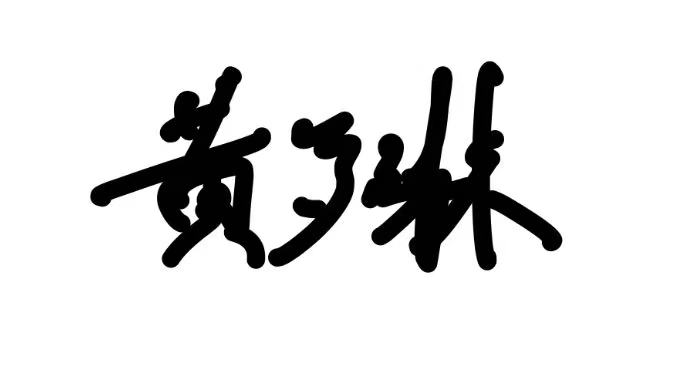
\includegraphics[width=1cm]{签字.jpg} & 评分: &\\
			\hline
			实验时间:& 2024/5/14 & 教师签名:&\\
			\hline
		\end{tabularx}
	\end{table}
	% ---
	
	% 小标题
	\section{全息照相实验  \quad\heiti 实验记录}
	% ---
	
	% 实验过程记录
	\subsection{实验内容、步骤与结果}
	
	%
	\subsubsection{操作步骤记录}
	\begin{enumerate}
		\item 激光器预热大约一个小时,以确保波长稳定。
		\item He-Ne 激光器发出的激光由分束镜分为两束,两束光强的比例要根据被摄物的漫反射能力以及参考光和物光在底片上的比例来决定。
		\item 参考光束和物光束都经过扩束镜扩束,移动扩束镜的位置(或改变扩束镜的倍率)可以放大或缩小光斑,从而在一定面积上的光强会增大或减小。
		\item 在底片位置处参考光束强度和物光束强度的比值可用光电池配以检流计在底片架上进行测量。
		\item 确认光路中物光和参考光的光程差大致相等;物光和参考光夹角在30-50°之间;物光和参考光光强比在3:1到5:1之间。
		\item 设定曝光时间进行曝光(注意在整个曝光时间内尽量避免走动及大声说话)。
		\item 关闭室内所有光源,在全暗条件下学会判断全息干板药膜面的方法。将全息干板药膜面面向被摄物体固定在干板架上。
		\item 拍摄完毕以后,全息片要经过显影、停影、定影、水漂及晾干等四个步骤以后才能观察再现,整个操作过程均应在暗绿灯下进行,要认真保持清洁。
		\item 底片处理完毕以后,就可以观察波前重建,得到的虚像。
	\end{enumerate}
	
	%
	\subsubsection{实验仪器摆放示意图}
	\begin{figure}[{H}]
		\centering
		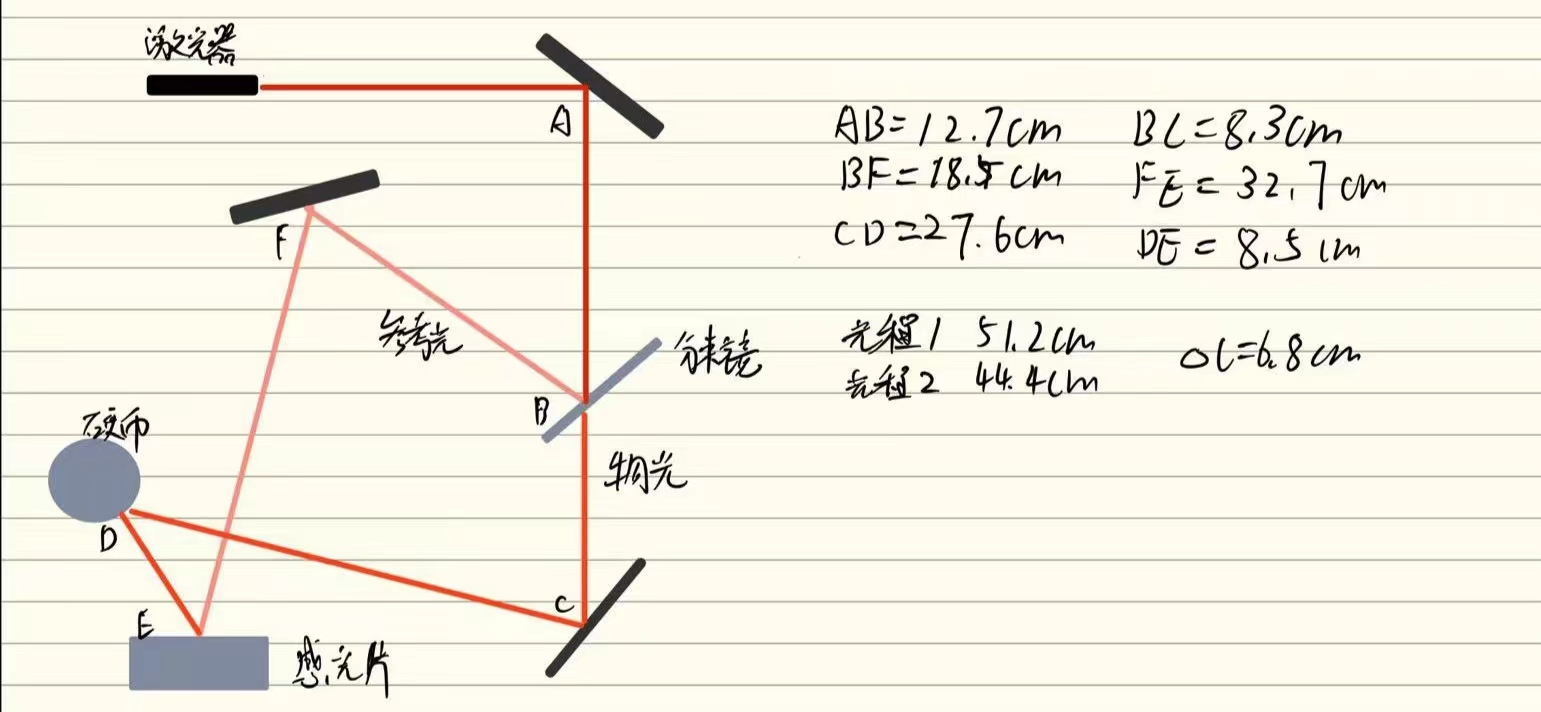
\includegraphics[width=0.8\linewidth]{示意图.jpg}
		\caption{仪器摆放示意图}
		\label{}
	\end{figure}
	光程差为6.8cm

	\subsection{失败原因分析}
	第一次实验我的确按照实验要求进行光路搭建,在后来移动光快门那个机器的屏幕的时候。我碰到了激光器……在实验中就会明显发现有一束光直接打在了我旁边的墙壁上……,然后就是一个可预见的失败了。

	第二次实验,我可能是因为在操作过程中吹的时间太长了,导致了实验的失败。
	
	不过对于我的第二次实验,还可能是因为我的光路的确出了问题,这个因为我可以肯定第二次实验的操作不至于导致一点像都看不到。

	光程差控制的相对较好,但是还是怀疑在某个环节出现了错误,当然,可能是我运气不好。

	当然如果有机会我还是想再做一次的,希望期末或者考完之后可以有机会再做一次,谢谢老师啦!!
	
	

	
	
	% 问题记录
	\subsection{实验过程遇到问题及解决办法}
	\begin{enumerate}
		\item 最严重的问题!!我没有调出来!!!
		\item 实验中出现了我对于两个光程的计算的错误,具体体现为我将最后一段的光在初次进行光程差计算时并没有加入到计算中。
		\item 在进行黑暗环境中的曝光的时候,我尽管做到没有触碰光学器具,但是我千不该万不该碰了激光器……这导致我的第一次曝光是一次可预见的失败……
		\item 实验中出现了第二次的问题是我在使用热吹风机的时候忘记那一边是药水面,所以我出现了反复吹了好久,导致了实验图像的无法再现。
		\item 至于对于是否在分束前进行扩束,由于如果提前扩束,会导致一部分光因为反射镜的大小影响而损失掉,所以我采用的是在最后进行两束光分别扩束。
	\end{enumerate}
	\begin{figure}[{H}]
		\centering
		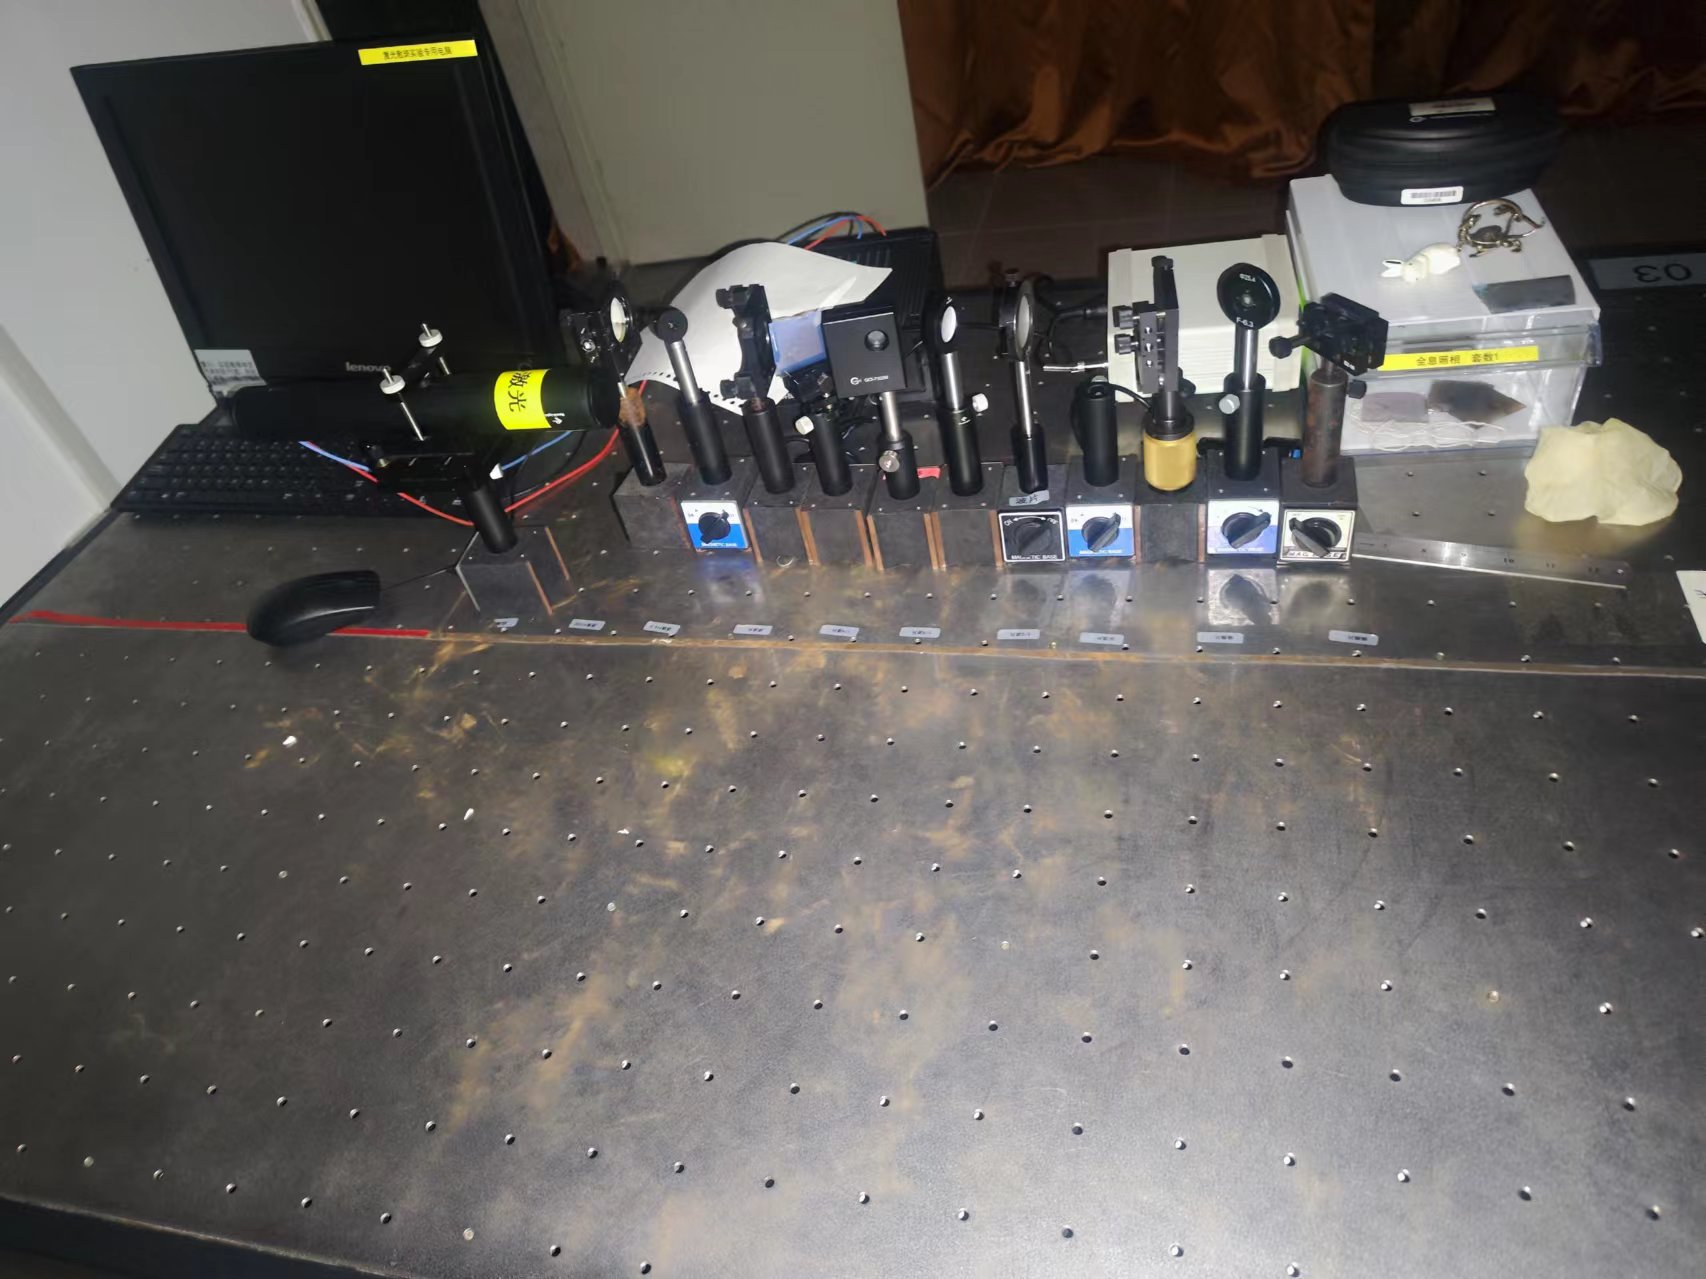
\includegraphics[width=0.4\linewidth]{桌面.jpg}
		\caption{桌面}
		\label{}
	\end{figure}
	
	
	
	
	
	
\end{document}